% !Mode:: "TeX:UTF-8"
\chapter{子宫肉瘤预后模型的数据提取}
\label{cha:data}

\section{数据源介绍}

数据提取过程如图\ref{fig:dataset1}所示:

\begin{figure}[!htbp]
    \centering
    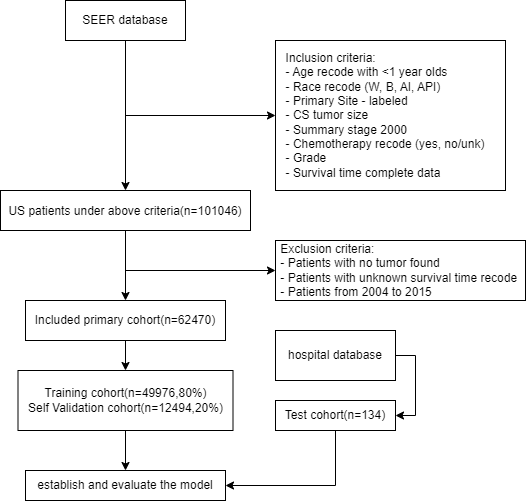
\includegraphics[scale=0.8]{paper_database.drawio.png}
    \caption{数据提取流程图} \label{fig:dataset1}
\end{figure}

由图可见,在SEER数据库中,首先提取从SEER数据库中提取数据,各字段信息将在后面的章节阐释如何筛选得到,最终得到数据101046条。然后通过排除标准,将SEERStat软件中中不能进行排除的部分不需要的数据进行脚本审查,最终分离得到需要的62470条训练用数据。将这些数据进行裁切,最后得到的是49976条训练数据与其附带的自验证数据12494条。

另一方面,由于SEER数据库中的数据存在一定局限性,其只包含被国立医学研究院认可并被SEER接收的数据。这意味着SEER的数据可能由于各地医疗情况与政策差异,不包含某些地区与特定人群的数据,如果文章使用SEER数据库进行验证,无疑会生成部分不够准确的研究内容,甚至影响将来的研究方向。因此,我从医院数据库中进行采集、梳理和标记,最后筛选得到134条验证数据,以供之后验证使用。这些数据可以验证或补充 SEER 数据,以确保研究结果的可靠性和准确性。而且从医院得到的数据也能帮助将来的研究者更好地了解特定疾病的治疗方案与效果,这些信息也会对将来的医学研究与实践具有重要的意义。

因此,使用 SEER 数据和从医院得到的数据都是重要的,以确保医学研究的结果更准确、全面和可靠。两者结合使用可以提高研究结果的可靠性和准确性,并为医学研究和实践提供更准确和有用的信息。

\subsection{SEER癌症数据库}

SEER(监测、流行病学和最终结果)计划提供大量癌症统计数据,它的目的是通过对癌症数据提供完整的监控数据,减少医疗系统中的癌症负担。SEER数据被认为是美国癌症研究的重要资源之一,因为它包括了来自不同地区的多种癌症类型的发病率和死亡率,以及提供了大量患者的年龄、性别、地理位置和治疗信息等详细信息,同时它也是国际公认的最大最成体系的癌症数据库之一。它起源于1971年美国国家癌症法(NCA)对于建立一个体系化数据库来收集、储存、分析和分发癌症相关数据,以用于支持、预防、诊断和治疗癌症的研究。SEER的病例收集从1973年1月1日开始,在美国的几个地理区间上进行诊断和提取。50年来SEER数据收集范围越来越大,同时内容也不断完整化、规范化,如今收集到的总数据已占美国人口的一半。大量来自不同种族和年龄段的癌症数据为研究者详细分析癌症提供了很大的便利。该数据集的优点是包含了多个癌症类型,且数据集中的样本数量较大,这使得研究人员可以更好地研究不同癌症类型的特点和趋势。

近年来,越来越多的研究人员开始使用该数据集来研究癌症分类和预测,每年大量有关癌症分类和预测的文章在各类期刊上发表,医学人士往往使用列线图等来提供可以在临床上进行定量使用的R语言模型,该数据集也被逐渐用于研究不同癌症类型的生物学特征和发病机制。

\subsection{医院验证数据库}

医院数据由我在医生老师们的指导下得到,如图\ref{fig:dataset_test_file}所示:

\begin{figure}[!htbp]
    \centering
    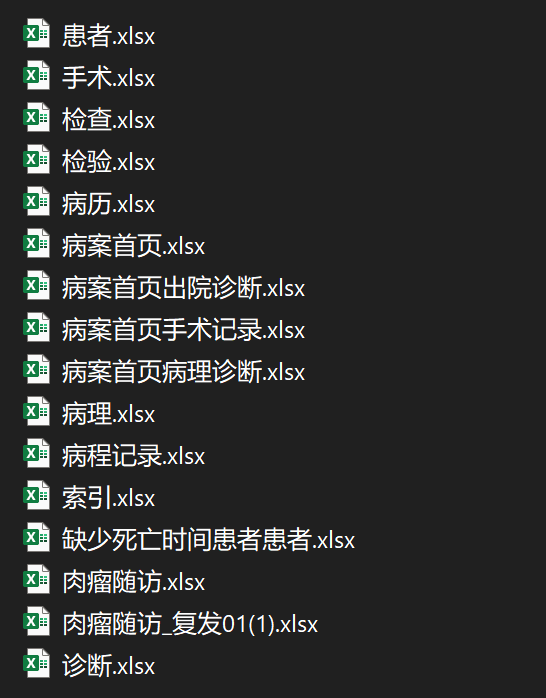
\includegraphics[scale=0.6]{hospital_dataset_files.png}
    \caption{医院原数据图} \label{fig:dataset_test_file}
\end{figure}

该数据库提供了患者的病例、检查等数据,在对其中字段内容进行遍历后,我比较了了训练数据中与验证数据中共同存在的一部分内容,并按照第\ref{cha:analyse}章分析结果确定最终纳入的变量。

\section{数据字段对应编码与含义}

从SEER数据集中,根据分析因素对生存率的相关性选择了下列字段:

\begin{figure}[!htbp]
    \centering
    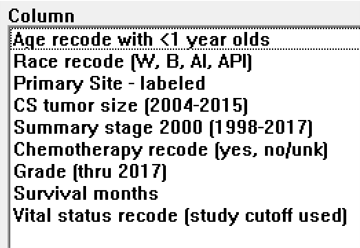
\includegraphics[scale=0.6]{seer_vals.png}
    \caption{SEERStat中选择的变量数据图} \label{fig:seer_vals}
\end{figure}

其中方括号内的时间段是由于编码方式改变产生,在不同的时间段有不同的编码方式,所以文章最终取交集2004-2015年范围间。
关于字段的解释如下:

\begin{itemize}
  \item 年龄(例:60-64 years)
  \item 种族(白人、黑人、美国印第安人/阿拉斯加原住民、亚洲人或太平洋岛民)
  \item 原发部位(子宫内膜、子宫肌层等)
  \item 肿瘤大小(最大直径)
  \item 肿瘤分期(Localized、Regional、Distant)
  \item 是否化疗(是、否/未知)
  \item 肿瘤分级(I、II、III、IV)
  \item 生存时间相关信息
\end{itemize}

文章中使用到的字段主要如上述列表所示。

首先,年龄使是以5年为一个单位所表示的,年龄重码变量是基于诊断时的年龄(单年年龄),使用的分组是由年龄决定的,年龄重新编码变量中使用的分组是由患者数据中的年龄分组决定的。这个重码变量中有19个年龄组(\textless1岁,1-4岁,5-9岁,...,85岁以上)。

第二个字段是种族,在SEER数据库中,主要有六个选项,他们分别是白种人、黑种人、美国印第安人/阿拉斯加原住民、亚洲人或太平洋岛民、其他未说明的(1991年以上)。考虑到在测试数据集中,我们使用的是中国人作为主要的测试患者,一开始我只使用了亚洲人或太平洋岛民的数据,但是在之后的模型建立中,我发现如果只使用亚洲人和太平洋岛民作为训练数据的话模型的效果并不好。可能的原因是亚洲人和太平洋岛民中存在着显出的差异,另一种可能的解释是数据量的不足。考虑到该字段频数的差异我最后使用了白种人黑种人和亚洲人或太平洋岛民作为训练集中开始算的参数选项。

文章使用的第三个字段是原发部位(Primary Site),这个字段主要表示病发的部位。这个字段提供了ICD-O-3规范的主要部位代码和一个描述性的主要部位标签该标签是首选的ICD-O-3加粗的名称,其他部位或子部位包含在代码中,但没有反映在代码中,本文使用的子宫肉瘤数据都包含ICD-O-3标签。编码中可能还包括其他部位或子部位,但没有反映在首选标签中。诊断年份在1992年之前的病例从早期版本转换为了ICD-O-3。这里亦只选取了四个选项,见图\ref{fig:seer_exclusion}中。

第四个字段是肿瘤大小,肿瘤大小指的是肉眼所见肿瘤的最大直径。肿瘤大小适用于2004-2015年的诊断年份。早期的病例部分会被转换,并增加新的编码以加以匹配,这些编码在目前的CS版本之前是不可用的,而且在当前版本的CS之前无法使用的新编码。关于肿瘤大小的详细说明见图\ref{fig:tumor_size}。

\begin{figure}[!htbp]
    \centering
    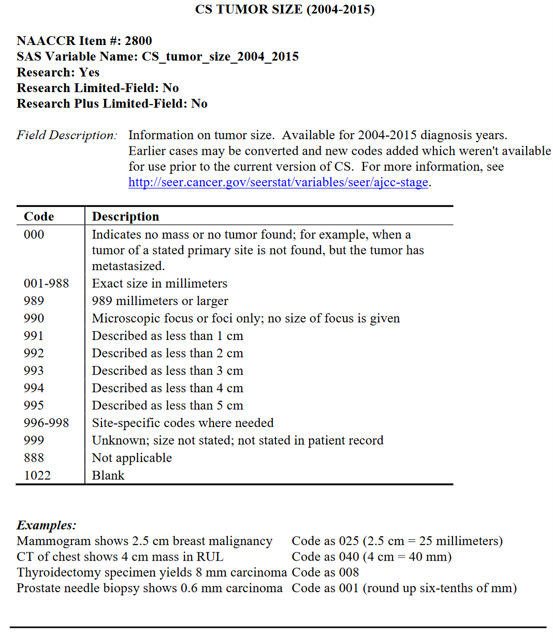
\includegraphics[scale=0.4]{tumor_size.png}
    \caption{SEER数据库中CS Tumor Size字段的详细说明图} \label{fig:tumor_size}
\end{figure}

肿瘤分期是指对恶性肿瘤进行分期分类的过程,它用于描述肿瘤的扩散程度和位置等特征,以便更好地评估肿瘤的严重程度和治疗前景。肿瘤分期通常由国际癌症联合会制定,其分期系统根据不同的肿瘤类型和特定癌症的组织学和生物学特征而有所不同。SEER主要使用的是TNM分期系统。TNM是一个在国际中广泛应用的为肿瘤进行而实现的系统,在它的分类标准中,主要针对以下几个方面进行分期:肿瘤的大小、淋巴的侵扰情况、肿瘤的转移与否。这里使用的是M标准,肿瘤的转移与否,主要分为三种情况,分别表示局部区域与远端三种类型。其中局部表示肿瘤仅限于原始的发生位置,没有扩散到周围组织或器官。区域表示肿瘤扩散到周围组织或病变器官,但没有扩散到远处的器官或淋巴结。远端则表示肿瘤已经扩散到其他远隔的器官或淋巴结。肿瘤分期表示了肿瘤扩散的进展过程,是对患者生存率有较大影响的一个影响因子。

化疗与否标识了患者是否使用了化疗作为辅助治疗手段。这里要主要的一点是由于患者隐私和机构编码原因,使用的两个编码分别是“是”和“否/未知”,这样的编码会对准确率产生一定的影响。

肿瘤分级是指对恶性肿瘤进行分期的的一种方法,它可以根据肿瘤的大小、形状、密度和边缘等特征来评估肿瘤的恶性程度。肿瘤分级通常由医生进行视觉评估,也可以通过计算机辅助断层扫描(CT)、磁共振成像(MRI)和其他影像学技术来进行辅助评估。这里一个分为四个等级:

\begin{itemize}
\item 等级一:这个等级是最低的,在这个等级中,肿瘤的分化情况最低,肿瘤细胞构成的组织和正常工作的组织差别较小,这种情况也常常被书面称为分化良好,肿瘤的恶性化程度最低。
\item 等级二:在这个等级中,肿瘤细胞已经开始出现一定的明显不同,这不但体现在肿瘤细胞的生长周期已经与正常细胞有明显的差异,而且肿瘤的形态也与其他组织有不同,这类组织恶性程度已经较高。
\item 等级三:这类肿瘤组织等级被称为分化最差的,这意味肿瘤的分化程度较差,大部分肿瘤细胞已经没有正常组织的功能表现了,内部是大量无定形的而无法描述的细胞,这类细胞由于分化程度低,所以增殖速度也最快,不成组织的细胞也最易向周围组织侵扰,所以危险程度也最高。
\item 等级四:这个等级表示未分化,这意味着肿瘤的分化程度最低,其中几乎没有分化的细胞,在临床中出现极少。
\end{itemize}

以上数据中,肿瘤大小、肿瘤分期、肿瘤分级与生存相关内容外的数据都可以直接使用SQL语句或Python脚本简单提取,这里我使用了ipynb文件作为提取方案,以适应研究过程中的大量更改。生存相关数据在数据库中并没有记录,所以我使用脚本筛选了所有提供联系方式的患者的信息,在医院方面进行随访后对得到的数据进行提取。

而肿瘤大小、肿瘤分期与分级数据没有直接字段提供,只能从病理分析中的诊断文本中提取,我首先筛选了其他字段记录完整的患者,并在这些数据的诊断信息中提取。肿瘤大小这里选取的是左附件区和右附件区中的最大肿瘤的最大直径,所以我编写了相应的Python 简单NLP算法,文本的左附件右附件的划分,并在这两段中分别找到用以描述肿瘤的大小。由于还有关于回声区和输卵管长度等的干扰,必须严格找到肿瘤对应的大小。最后在得到的所有肿瘤大小中找到最大值并返回。无匹配内容的描述只能得到空值作为回应,所以最后我对所有数据进行了人工校验。而肿瘤分期与分级同理,先在文本中检索是否有直接指明的描述,如果没有则按照上文中的定义来确定相应的内容。

通过上述的处理,初步筛选得到的300条数据在去除上述内容的缺失后一共是134条测试数据。

\begin{figure}[!htbp]
    \centering
    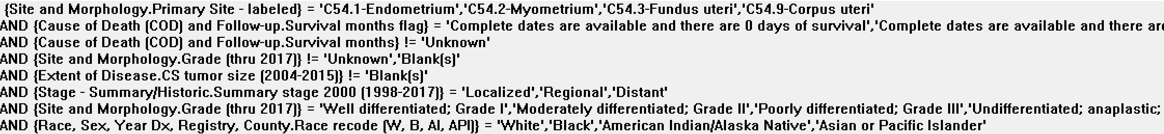
\includegraphics[scale=0.4]{seer_exclusion.png}
    \caption{SEERStat中选择的变量排除条件图} \label{fig:seer_exclusion}
\end{figure}
